\PassOptionsToPackage{svgnames}{xcolor}
\documentclass[12pt]{article}



\usepackage[margin=1in]{geometry}  
\usepackage{algorithm,algpseudocode}
\newcommand{\vars}{\texttt}
\newcommand{\func}{\textrm}
\usepackage{graphicx}             
\usepackage{amsmath}              
\usepackage{amsfonts}
\usepackage{framed}               
\usepackage{amssymb}
\usepackage{array}
\usepackage{amsthm}
\usepackage{multirow}
\usepackage[nottoc]{tocbibind}
\usepackage{bm}
\usepackage{enumitem}
\usepackage{tikz}
\usepackage{pdfpages}
\usepackage{tabularx}
\algdef{SE}[SUBALG]{Indent}{EndIndent}{}{\algorithmicend\ }%
\algtext*{Indent}
\algtext*{EndIndent}
\newcolumntype{C}[1]{>{\centering\let\newline\\\arraybackslash\hspace{0pt}}m{#1}}
\newcommand\norm[1]{\left\lVert#1\right\rVert}
\setlength{\parindent}{0cm}
\setlength{\parskip}{0em}
\newcommand{\ind}{\hspace*{15pt}}
\newcommand{\Lim}[1]{\raisebox{0.5ex}{\scalebox{0.8}{$\displaystyle \lim_{#1}\;$}}}
\newtheorem{definition}{Definition}[section]
\newtheorem{theorem}{Theorem}[section]
\newtheorem{notation}{Notation}[section]
\theoremstyle{definition}
\DeclareMathOperator{\arcsec}{arcsec}
\DeclareMathOperator{\arccot}{arccot}
\DeclareMathOperator{\arccsc}{arccsc}
\DeclareMathOperator{\spn}{Span}
\DeclareMathOperator{\diff}{d}
\setcounter{tocdepth}{1}
\begin{document}
\title{Revision notes - CS4246}
\author{Ma Hongqiang}
\maketitle
\tableofcontents

\clearpage
%\twocolumnt
\section{Deterministic Planning}
\subsection{Problem Solving}
\begin{definition}[Problem]
\hfill\\\normalfont A \textbf{problem} is defined by 5 components:
\begin{enumerate}
	\item \textbf{Initial State}
	\item Possible \textbf{Actions}. $\textsc{Action}(s)$ returns set of actions that can be executed in $s$.
	\item \textbf{Transition model}. $\textsc{Result}(s,a)$ returns state that results from doing $a$ in $s$.\\ The sets of all states reachable from the initial state is called the state space. Transitional model forms a directed graph over all the states.
	\item \textbf{Goal test}.
	\item \textbf{Path Cost}. Often it is the sum of the step cost, $c(s,a,s')$.
\end{enumerate}
\end{definition}
When the number of states is not too large, we can solve the optimal path by using the \textsc{Uniform-Cost-Search}. \\
$A^\ast$ search is the same as \textsc{Uniform-Cost-Search} except that it uses $f(n):=g(n)+h(n)$ to sort the priority queue, where
\begin{itemize}
	\item $g(n)$ is the cost to reach node $n$
	\item $h(n)$ is a \textbf{heuristic} that estimates the cheapest cost from $n$ to the goal state
\end{itemize}
\begin{theorem}[Optimality of {$A^\ast$}]
\hfill\\\normalfont $A^\ast$ is optimal under tree search if $h(n)$ is admissble, i.e., $h$ never overestimates the cost to the goal.\\
$A^\ast$ is optimal under graph search if $h(n)$ is consistent, i.e., 
\[
h(n)\leq c(n,a,n')+h(n')
\]
where $c(n,a,n')$ is the cost for going from $n$ to $n'$ using $a$.
\end{theorem}
Generally, admissible heuristics comes from a \textit{relaxed} problem, where there are fewer restrictions on the actions.
\begin{definition}[Domination]
\hfill\\\normalfont We say $h_2$ dominates $h_1$ if $h_2(n)\geq h_1(n)$ for all $n$ in state space.
\end{definition}
If $h_2$ dominates $h_1$, $h_2$ will \textit{always} explore fewer nodes with $A^\ast$.\\
Generally, one useful property to identify the heuristic is as below: suppose $S\subseteq \Omega$, and there is $f:\Omega\to \mathbb{R}$. Then, we have
\[
\inf f(S) \geq f(\Omega)
\]
Here, $S$ is the state of the problem and $\Omega$ an relaxed problem, where $f$ is the function that maps states to heurstic's costs.\\

However, when state space is defined in terms of state variables, i.e. \textbf{factored representation}, it is usually exponentially large with respect to the number of variables. Therefore, $A^\ast$ algorithm will run out of memory as it stores all states. In such cases, \textbf{depth first search} should be used, which only requires $O(m)$ memory, where $m$ is the depth of the search.\\
Other variants of depth-first search includes \textbf{iterative deepening search} and \textbf{iterative deepening} $A^\ast$.
\subsection{Classical Planning}
Classical planning usually uses a language called \textbf{Planning Domain Definition Language}(PDDL), in which 
\begin{itemize}
	\item Initial state,
	\item Actions available in a state,
	\item Result of applying an action
	\item Goal test
\end{itemize}
are defined.
\begin{definition}[State]
\hfill\\\normalfont A \textbf{state} is a conjunction of fluents.\\
\textbf{Fluents} are state variables, representing variables that can change through time. In PDDL, fluents are \textbf{ground boolean variables}.\\
A state is then a \textbf{conjunction of fluents}.
\end{definition}
In description of state, \textbf{database semantics} are used where
\begin{itemize}
	\item Fluents not mentioned are false, because of the closed world assumption.
	\item Unique name assumption, which means variable of distinct names are distinct.
\end{itemize}
The state description forbids the below scenarios:
\begin{itemize}
	\item $\text{At}(x,y)$, as the boolean variable is not grounded
	\item $\neg\text{Poor}$ because of the negation
	\item $\text{At}(\text{Father}(\text{Fred}), \text{Sydney})$ because PDDL does \textit{not} allow functions.
\end{itemize}
\begin{definition}[Action Schema, Action]
\hfill\\\normalfont A set of actions is specified by an \textbf{action schema}, which is a \textbf{lifted representation}, lifted from propositional logic to a restricted subset of \textit{first order} logic.\\
A schema consists of 
\begin{enumerate}
\item an action name,
\item a list of all variables
\item a precondition
\item an effect
\end{enumerate} 
By instantiating the variables, a schema can give \textbf{ground actions}.\\
The precondition and effect are conjunctions of literals(positive or negative atmoic sentences). Here, precondition specifies states where the action can be executed: action $a$ is \textbf{applicable} in state $s$ if the preconditions are satisfied by $s$.
\end{definition}
A set of action schemas defines a planning domain.
\begin{definition}[Result]
\hfill\\\normalfont The \textbf{result} of executing action $a$ in state $s$ is a state $s'$ which is a set of fluents formed as follows:
\begin{itemize}
	\item Start from $s$
	\item Remove fluents that appears in teh action's effect as negative literals
	\item Add fluents that appear in the action's effect as positive literals
\end{itemize}
\[
\textsc{Result}(s,a) = (s-\textsc{Del}(a))\cup\textsc{Add}(a)
\]
\end{definition}
\begin{definition}[Initial State, Goal]
\hfill\\\normalfont A specific problem is defined by adding an initial state and a goal, where
\begin{enumerate}
	\item The \textbf{initial state} is a conjunction of ground atoms.
	\item The \textbf{goal state} is conjunction of literal, positive or negative, that may contains variables.
\end{enumerate}
\textbf{Remark}: Variables are treated as existentially quantified.
\end{definition}
Solution to a planning problem is essentially a path from initial state to goal. We can find this path from 
\begin{enumerate}
	\item Forward search
	\item Backward search
\end{enumerate}
Forward search has the problem of 
\begin{itemize}
\item large state space, which is exponential to the number of state variables.
\item Large action space
\end{itemize}
but there exists strong domain independent heuristics that can be automatically derived, which makes forward search feasible for many problems.\\

In contrast, backward search, also called \textbf{relevant-state} search, only considers actions that are relevant to the goal, or current state. To formalise this, we distinguish state and description:
\begin{definition}[State, Description]
\hfill\\\normalfont In a state, every variable is assigned a value. Therefore, for $n$ ground fluents, there are $2^n$ ground states.\\
However, for $n$ ground fluents, there are $3^n$ descriptions, as each fluent can be positive, negative or not mentioned.\\
We can use description with omitted fluent to describe a set of states.
\end{definition}
In backward search, we regress from a state description to a predecessor state description.
\begin{theorem}[Regression in PDDL]
\hfill\\\normalfont Given goal $g$ and action $a$, regression from $g$ over $a$ gives description $g'$, where
\[
g'=(g-\textsc{Add}(a))\cup\text{Precondition}(a)
\]
\end{theorem}
For backward search, we want actions used for regression to be \textbf{relevant}, in the following sense.
\begin{definition}[Relevant Action]
\hfill\\\normalfont An action is relevant if
\begin{enumerate}
	\item At least 1 of the action's effect must unify with an element of the current goal
	\item Must not have any effect that negate an element of the current goal
\end{enumerate}
When unifying, we substitute the most general unifier in the regressed state $g'$, to keep the branching factor down without ruling out any solution.
\end{definition}
\subsubsection{Heuristics for Foward Search}
\begin{definition}[Ignore Pre-condition Heuristic]
\hfill\\\normalfont \textbf{Ignore Pre-condition Heuristic} drops all pre-conditions.\\
Since it solves a relaxed problem, it never overestimates, which makes it admissible.\\
Number of steps is roughly number of unsatisfied goals, except some actions that can satisfy multiple goals, or undo some goals.\\

If relaxed further to remove all effects except literals in teh goal, problem becomes minimum number of actions, such that the union of effects satisfies the goal, which is known as \textbf{set cover problem}, a $NP$-hard problem. However, it is known that there is a $\log n$-approximation algorithm for set cover.
\end{definition}
\begin{definition}[Ignore Delete List Heuristic]
\hfill\\\normalfont \textbf{Ignore Delete List Heuristic} assumes goal and pre-condition contains only positive literals. Then this heuristics allows monotonic progress towards goal.\\
Since it is a relaxed problem, it is admissible. However, the relaxed problem is still $NP$-hard, and hill climbing gives an approximate solution.
\end{definition}
\begin{definition}[Problem Decomposition]
\hfill\\\normalfont If we can divide goal $g$ into $g_1,\ldots, g_n$ subgoals, which $a_1,\ldots, a_n$ can be used to solve. If each subproblem uses an admissible heuristic, then \textbf{taking max} is admissible.\\
Furthermore, if we assume \textbf{subgoal independence}, then sum of the cost of solving each subgoal
\begin{itemize}
	\item is optimistic when there is negative interaction
	\item is pessimistic when there is positive interaction, thus inadmissible.
\end{itemize}
If the sum is admissible, then it will be a better heuristic than taking max.
\end{definition}
\subsection{SATPlan}
One way to do planning is to transform the planning problem into a \textbf{Boolean satisfiability}(SAT) problem, and solve using a SAT solver.\\
It is known that SAT is $NP$-complete, but SAT solvers are effective in practice by exploiting various heuristics.\\

Solving SAT requires finding an assignment to variables that will make a Boolean formula TRUE, or declare no assignment exists.\\

SAT solvers usually takes input in Conjunctive Normal Form(CNF) which is a conjunction of disjunction of literals. It is known that any boolean formula can be converted into CNF.

\begin{theorem}[Translate PDDL into SAT]
\hfill\\\normalfont We need the following steps to translate PDDL to SAT:
\begin{enumerate}
\item Propositionalise the actions, by replace each action schema with the set of ground actions by substituting constants for each variable.
\item Define initial state: assert $F^0$ for every fluent $F$ in initial state and $\neg F^0$ for every fluent not in initial state. \footnote{Superscript denotes the time.}
\item Propositionalise the goal: each goal is a conjunction. Therefore, the propositionalised goal should be a disjunction over all possible ground conjunctions obtained by replacing variables with constants.
\item Add \textbf{successor-state} axioms. For each fluent $F$, add axiom of the form
\[
F^{t+1}\Leftrightarrow \text{ActionCauses} F^t \lor (F^t\land \neg \text{ActionCausesNot} F^t)
\]
where ActionCasues$F^t$ is a disjunction of all ground actions that have $F$ in \textsc{Add} list, and ActionCausesNot$F^t$ is a disjunction of all ground actions that have $F$ in \textsc{Del} list.\\
Note, this is a better substitutes to frame axioms, which looks like $A\Rightarrow (F^t\Leftrightarrow F^{t+1})$, for all $A$ and $F$, as it will have fewer number of total axioms.
\item Add \textbf{preconditon} axioms: for each ground action $A$, add axiom $A^t\Rightarrow \textsc{Pre}(A)^t$. Equivalently speaking, if an action is taken at time $t$, its preconditions must have been true at time $t$.
\item Add \textbf{action exclusion} axioms: every action is distinct from every other actions, i.e. only one action is allowed at each time step. It is in the form $\neg A_i^t\lor \neg A_j^t$ for all pairs of $i,j$.\\
If we want to allow parallel action, add mutual exclusion only if the pair of action really interfere with each other
\end{enumerate}
\end{theorem}
We have defined the translation process. The general algorithm of SATPlan is defined below:
\begin{theorem}[{\textsc{SATplan}}]
\hfill\\\normalfont
\textbf{function} \textsc{SATplan}(\textit{init},\textit{transition},\textit{goal},$T_{\max}$) \textbf{returns} solution or failure\\
\ind\textbf{inputs}: \textit{init},\textit{transition},\textit{goal}, constitute a description of the problem\\
\ind$T_{\max}$, an upper limit of plan length\\

\ind\textbf{for} $t=0$ \textbf{to} $T_{\max}$ \textbf{do}\\
\ind\ind\textit{cnf}$\leftarrow$\textsc{Translate-To-SAT}(\textit{init},\textit{transition},\textit{goal},$t$)\\
\ind\ind\textit{model}$\leftarrow$\textsc{SAT-Solver}(\textit{cnf})\\
\ind\ind\textbf{if} \textit{model} is not null \textbf{then}\\
\ind\ind\ind\textbf{return} \textsc{Extract-Solution}(\textit{model})\\
\ind\textbf{return} \textit{failure}
\end{theorem}

\section{Decision Theory}
\begin{definition}[Rationality of Agent]
\hfill\\\normalfont A \textbf{rational} agent is the one that chooses the action that maximises its \textbf{expected utlity}. Specifically, we want to maximize the expected utility of action $a$ given evidence $e$
\[
EU(a\mid e) := \sum_{s'} P(\textsc{Result}(a)=s'\mid a,e)U(s')
\]
where $P(\textsc{Result}(a)=s'\mid a,e)$ is the probability of outcome $s'$ given that action $a$ and evidence $e$, and $U(s)$ is \textbf{utility function} assigning a number to indicate desirability of state $s$.
\end{definition}
\subsection{Utility Theory}
We take an axiomatic approach to define utility. We first adopt a few axioms that defines preferences between outcomes' behaviours, and utlities arise as the consequence of the preferences.

Here, we assume that agent has the following three types of preferences, namely
\begin{itemize}
	\item $A\succ B$: agent prefers $A$ over $B$
	\item $A\sim B$: agent is indifferent between $A$ and $B$
	\item $A\succsim B$: agent prefers $A$ over $B$ or is indifferent
\end{itemize}
Here $A$, $B$ may be either states of the world, which is deterministic, or \textbf{lottery}, whose outcome is not deterministic.
\begin{definition}[Lottery]
\hfill\\\normalfont A \textbf{lottery} $L$ with outcome $S_1,\ldots, S_n$ that occurs with probabilities $p_1,\ldots, p_n$ is denoted as
\[
L=[p_1,S_1;p_2,S_2;\ldots;p_n,S_n]
\]
\end{definition}
\begin{theorem}[Axiom of Utility Theory]
\hfill\\\normalfont There are 6 axioms that constitutes the \textbf{axioms of utility theory}. They are
\begin{enumerate}
	\item \textbf{Orderability}: Given any two lotteries, a rational agent must rate with one of three possibilities:
	\begin{enumerate}
		\item Prefer one: $A\succ B$
		\item Prefer the other: $B\succ A$
		\item Prefer two equally: $A\sim B$
	\end{enumerate}
	\item \textbf{Transitivity}: If the agent prefers $A$ to $B$ and $B$ to $C$, then the agent must prefer $A$ to $C$
	\[
(A\succ B)\cap (B\succ C)\Rightarrow (A\succ C)
	\]
	\item \textbf{Continuity}: If $B$ is between $A$ and $C$ in preference, there must be a $p$, such that the agent is indifferent to getting $A$ with probability $p$ and $C$ with probability $(1-p)$.
	\[
A\succ B\succ C \Rightarrow \exists p [p,A; 1-p, C]\sim B
	\]
	\item \textbf{Substitutability}: If an agent is indifferent between two lotteries $A$ and $B$, then the agent is indifferent to two complex lotteries that are the same, except $B$ is substituted for $A$:
	\[
A\sim B\Rightarrow [p,A; 1-p,C]\sim [p,B; 1-p,C]
	\]
	The above condition also holds if $\succ$ is substituted for $\sim$.
	\item \textbf{Monotonicity}: Suppose two lotteries have the same two possible outcomes, $A$ and $B$. If an agent prefers $A$ to $B$, the agent must prefer the lottery that has higher probability for $A$, and vice versa.
	\[
A\succ B \Rightarrow (p>q) \Leftrightarrow [p,A; 1-p, B]\succ [q,A; 1-q, B]
	\]
	\item \textbf{Decomposibility}: Compound lotteries can be reduced to simpler ones using the law of probability.
	\[
[p,A; 1-p[q,B; 1-q, C]] \sim [p,A; (1-p)q, B; (1-p)(1-q), C]
	\]
\end{enumerate}
\end{theorem}
\begin{theorem}[Existence of Utility Function]
\hfill\\\normalfont If agent's preferences obey the axioms of utlity, then there exists a function $U$ s.t. $U(A)>U(B)$ iff $A$ is preferable to $B$ and $U(A)=U(B)$ iff agent is indifferent between $A$ and $B$.
\[
U(A)>U(B)\Leftrightarrow A\succ B
\]
\[
U(A)=U(B)\Leftrightarrow A\sim B
\]
\end{theorem}
\begin{theorem}[Expected Utility of a Lottery]
\hfill\\\normalfont The utility of a lottery is the expected value of the utility function
\[
U([p_1,S_1; \ldots; p_n, S_n]) = \sum_i p_iU(S_i)
\]
\end{theorem}
With the above setup, we have the following result:
\begin{theorem}
\hfill\\\normalfont An agent can act rationally only by choosing an action that \textbf{maximizes the expected utility}. If not, it will violate some of the axioms of utility.
\end{theorem}
Also, do note that 
\begin{itemize}
\item an agent's behaviour does not change if the utility function is transformed an affine transformation $U'(S)=aU(S)+b$ with $a>0$.\\
\item In a deterministic environment, a monotonic increasing transformation also does not change behaviour.
\item In a deterministic environment, only the axiom of orderability and transitivity is required, as other axioms all involve lotteries.
\end{itemize}
\subsection{Utility Function}
Process of presenting choices to agents and working out the utility function from observed responses is often called \textbf{preference elicitation}.\\
Usually, for \textbf{normalised utilities},we
\begin{enumerate}
	\item Fix values $u_{\bot} = 0$ and $u_{\top} = 1$.
	\item For any other prize $S$, we ask agent to choose between prize and a \textbf{standard lottery} $[p,u_{\bot}; 1-p, u_{\top}]$
	\item Adjust $p$ until agent is indifferent between $S$ and lottery, which is the utility of $S$.
\end{enumerate} 
However, by Arrow's Impossibility Theorem, utilities of a group cannot be fairly determined. 
\subsubsection{Utility of Money}
An agent ususally prefers money more than less; we say the preference of money is \textbf{monotonic preference}.\\
However, most people are risk averse($U''<0$), on positive part of curve; and risk seeking on large negative wealth($U''>0$).\\
To have a clearer representation of the value of a lottery in the eye of some agent, We can measure the value an agent will accept in lieu, which is defined as the \textbf{certainty equivalent} of the lottery.\\
The difference between Expected Monetary Value and its certainty equivalent is the \textbf{insurance premium}.\\
Since utility theory is a normative theory, there can be reallife scenarios where people act irrationally, as people fall into
\begin{itemize}
	\item \textbf{Certainty effect}, where they are strongly attracted to gains that are certain, and choose not to gamble due to possible regrets
	\item \textbf{Ambiguity aversion}, where they prefer known probability to unknown ones
	\item \textbf{Framing Effect}, where exact wording of choices have big impacts on choices
	\item \textbf{Anchoring effect}, where they prefer to make relative utility judgements to absolute ones
\end{itemize}
\subsection{Multiattribute Utility Function}
When outcomes are characterised by two or more attributes, we employ multiattribute utility theorey, where we have
\begin{itemize}
	\item Attribute $\bm{X}=X1,\ldots, X_n$
	\item Assignment $\bm{x}=\langle x_1,\ldots, x_n\rangle$.
	\item with ordering of values for $x_i$, and higher value of attribute implying higher utilityu
\end{itemize}
\begin{definition}[Strict Dominance]
\hfill\\\normalfont Option $A$ strictly dominates $B$ if $B$ has lower value on all attributes than $A$'s. If $A$ and $B$ are uncertain, $A$ strictly dominates $A$ if any value of $A$ can strictly dominates all possible values of $B$.
\end{definition}
\begin{definition}[Stochastic Dominance]
\hfill\\\normalfont $A_1$ is stochastically dominating $A_2$ on $X$ if
\[
\forall x, \int_{-\infty}^x p_1(x')\diff x'\leq \int_{-\infty}^xp_2(x')\diff x'
\]
\end{definition}
\begin{definition}[Preference Independent]
\hfill\\\normalfont An attribute $X_1$ is \textbf{preference independent}(PI) of $X_2$ if
\[
\langle x_1,x_2^0\rangle \succ\langle x_1',x_2^0\rangle \Rightarrow \langle x_1,x_2\rangle \succ\langle x_1',x_2\rangle \text{ for all } x_2
\]
In other words, preference of $x_1$ does not depend on value of $x_2$.
\end{definition}
We say atrributes $A$ are mutually preference indepdendent(MPI) if any subset $X\subseteq A$ is preference independent of its complement $Y=A\setminus X$.\\
If $A$ is MPI, there exists an \textbf{additive preference function} where there is no uncertainty
\[
V(x_1,\ldots, x_n)=\sum_{i=1}^n V_i(x_i)
\]
\begin{definition}[Utility Independent]
\hfill\\\normalfont We say a set of attributes $\bm{X}$ is utility independent $\bm{Y}$ if preferences between lotteries on $\bm{X}$ are independent of values of $\bm{Y}$.\\
A set of attributes is mutually utility independent if each of its subset is utility independent of the remainder.
\end{definition}
MUI implies a multiplicative utility function $U=k_1U_1+k_2U_2+k_3U_3+k_1k_2U_1U_2+k_2k_3U_2U_3+k_3k_1U_3U_1+k_1k_2k_3U_1U_2U_3$ for a set of 3 attributes.
\subsection{Decision Network}
\begin{definition}[Decision Network]
\hfill\\\normalfont Decision netowrk combine Bayesian network with additional nodes to denote actions and utilities.
\begin{figure}[h]
\centering
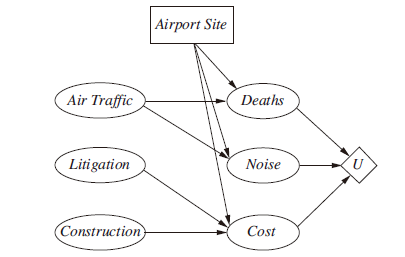
\includegraphics[width=0.5\textwidth]{1.png}
\end{figure}
\begin{itemize}
	\item \textbf{Chance nodes}, in oval, represent random variables. It should have a conditional distribution given its parent.
	\item \textbf{Decision Nodes}, in rectangle, represents points where dicision maker has a choice of actions.
	\item \textbf{Utility nodes}, in diamonds, represent the utility function. Its parent are all the variables that directly affect the utility.\\Utility node is associated with \textbf{action-utility function}, representing expected utility associated with each action. 
\end{itemize}
\end{definition}
In choosing an action, we
\begin{itemize}
	\item Set evidence variable to the \textit{observed} states
	\item For each possible value of the decision node
	\begin{enumerate}
		\item Set decision node to that value
		\item Calculate posterior probability of parents of utility node
		\item Calculate resulting utility of this action
	\end{enumerate}
	\item Return action with highest utility
\end{itemize}
\subsection{Value of Information}
Assume exact evidence can be obtained about variable $E_j$, we can compute the \textbf{value of perfect information}(VPI), in three steps:
\begin{itemize}
	\item Given current evidence $\mathbf{e}$, compute expected utility with current best action $\alpha$
	\[
EU(\alpha\mid \mathbf{e})=\max_a\sum_{s'} P(\textsc{Result}(a)=s'\mid a, \mathbf{e})U(s')
	\]
	\item Value of best new action after $E_j=e_j$ is obtained
	\[
EU(\alpha_{e_j}\mid \mathbf{e},e_j)=\max_a\sum_{s'}P(\textsc{Result}(a)=s'\mid a, \mathbf{e},e_j)U(s')
	\]
	\item Variable $E_j$ can take multiple values $e_{jk}$, so must average:
	\[
VPI_{\mathbf{e}}(E_j)=(\sum_{k} P(E_j=e_{jk}\mid\mathbf{e})EU(\alpha_{e_{jk}}\mid \mathbf{e},e_{jk}))-EU(\alpha\mid \mathbf{e})
	\]
\end{itemize}
We have the following properties on VPI:
\begin{itemize}
	\item Expected value of information is non-negative:
	\[
\forall \mathbf{e},E_j\;\;\;VPI_\mathbf{e}(E_j)\geq 0
	\]
	\item VPI is not additive
	\[
VPI_\mathbf{e}(E_j,E_k)\neq VPI_\mathbf{e}(E_j)+VPI_\mathbf{e}(E_k)
	\]
	\item VPI is order independent
	\[
VPI_\mathbf{e}(E_j,E_k) = VPI_\mathbf{e}(E_j)+VPI_{\mathbf{e},e_j}(E_k)= VPI_\mathbf{e}(E_k)+VPI_{\mathbf{e},e_k}(E_j)
	\]
\end{itemize}
Generally, as expected value of information is non-negative, agents should gather information before taking actions, if possible.
\clearpage
\section{Markov Decision Process}
\begin{definition}[Markov Decision Process]
\hfill\\\normalfont A markov decision process consists of a tuple $(S,A,T,R)$ where
\begin{itemize}
\item $S$, a set of states, with initial state $s_0$ specified
\item $A$, a set of actions
\item $T$, a transition model, defined by $P(s'\mid s,a)$.
\item $R$ a reward function, in $R(s,a,s')$.
\end{itemize} 
A transition model is a model that describes the probability of reaching state $s'$ if action $a$ is done in state $s$, i.e. $P(s'\mid s,a)$. \textbf{Markovian} assumption is applied here: probability depends only on state $s$ but not history of states earlier.\\
A reward function is a utility function that depends on \textit{sequence of }states. More details will be provided later.\\
\end{definition}
\begin{definition}[Policy]
\hfill\\\normalfont A \textbf{policy} $\pi(s)$ is a function from state to action.\\
Quality of policy is measured by \textbf{expected utility of possible environment histories generated by the policy}. Therefore, \textbf{optimal policy} $\pi^\ast$ is a policy that generates highest expected utility.
\end{definition}
\begin{definition}[Finite Horizon, Infinite Horizon]
\hfill\\\normalfont In a \textbf{finite horizon} problem, there is a fixed time $N$, after which nothing matters. Therefore, optimal action at a given state can change over time, i.e., optimal policy is \textbf{nonstationary}.\\
In an \textbf{infinite horizon} problem, there is no fixed time limit; optimal action depends only on current state, and therefore \textbf{stationary}.
\end{definition}
There are only two coherent ways to assign utilities: 
\begin{enumerate}
	\item Additive Rewards:
	\[
U_h([s_0,s_1,\ldots, ])=R(s_0)+R(s_1)+\cdots
	\]
	\item Discounted rewards:
	\[
U_h([s_0,s_1,\ldots, ])=R(s_0)+\gamma R(s_1)+\gamma^2 R(s_2)+\cdots
	\]
	where $\gamma$ is a discount factor between 0 and 1.
\end{enumerate}
Suppose we have maximum reward bounded by $\pm R_{\max}$, then the discounted rewards will be bounded by $\frac{R_{\max}}{1-\gamma}$ whereas additive rewards will be unbounded, if the problem has infinite horizon. Therefore, discounted rewards is recommended.
\begin{definition}[Proper Policy]
\hfill\\\normalfont In environment with terminal states and policies that are guaranteed to terminate, we can use $\gamma=1$. A policy that is guaranteed to terminate is called \textbf{proper policy}.\\
\end{definition}
Also, infinite sequences can be compared using average reward per unit time.
\begin{definition}[Expected Utility under discounted rewards]
\hfill\\\normalfont Expected utility of executing $\pi$ starting from $s$ is
\[
U^\pi(s)=E[\sum_{t=0}^\infty \gamma^t R(S_t)]
\]
with $S_0=s$, where the expectation is taken with respect to distribution of state sequ3ences determined by $\pi$ and $s$.
\end{definition}
Therefore, optimal policy $\pi_s^\ast$ is given by $\pi_s^\ast=\arg\max_{\pi} U^{\pi}(s)$.\\
In case of there are $n$ states and $a$ actions, the number of policies are $a^n$ which is bounded. Therefore, the optimal policy can always be determined.
\begin{definition}[Value Function]
\hfill\\\normalfont The utility of a state $s$ under optimal policy $U^{\pi^\ast}(s)$ is called the \textbf{value function}.
\end{definition}
Given the value function, the optimal policy can be determined by
\[
\pi^\ast(s)=\arg\max_{a\in A(s)}\sum_{s'} P(s'\mid a,s)U(s')
\]
The problem is that $U$ requires information of $\pi^\ast(s)$ for all $s$. Therefore, we need techinques to get $U$.
\subsection{Value Iteration}
\begin{definition}[Bellman Equation]
The Bellman equation states, the utility of a state is its immediate reward plus expected utility of next states, given optimal action
\[
U(s)=R(s)+\gamma\max_{a\in A(s)}\sum_{s'}P(s'\mid s,a)U(s')
\]
\end{definition}
\begin{theorem}[Value Iteration Algorithm]
\hfill\\\normalfont Value Iteration Algorithm returns a utility function that is $\epsilon$ close to the actual utility function.

\textbf{function} \textsc{Value-Iteration}(\textit{mdp},$\varepsilon$) \text{returns} a utility function\\
\ind\textbf{inputs}: \textit{mdp}:=$(S,A,P,R)$ and discount $\gamma$.\\
\ind\ind reward $\varepsilon$, the maximum error allowed in utility of any state\\
\ind\textbf{local variables}: $U,U'$ vectors of utilities for state in $S$, initially zero\\
\ind\ind $\delta$, the maximum change in the utility of any states in an iteration\\
\ind\textbf{repeat}\\
\ind\ind $U\leftarrow U'$, $\delta\leftarrow 0$\\
\ind\ind \textbf{for each} state $s$ \textbf{in} $S$ \textbf{do}\\
\ind\ind\ind $U'[s]\leftarrow R(s)+\gamma\max_{a\in A(s)}\sum_{s'}P(s'\mid a,s) U[s']$\\
\ind\ind\ind\textbf{if} $|U'[s]-U[s]|>\delta$ \textbf{then} $\delta\leftarrow |U'[s]-U[s]|$.\\
\ind\textbf{until} $\delta<\varepsilon(1-\gamma)/\gamma$
\ind\textbf{return} $U$.
\end{theorem}
Essentially, the above algorithm repeatedly apply \textbf{Bellman update}
\[
U_{t+1}(s)=R(s)+\gamma\max_{a\in A(s)}\sum_{s'}P(s'\mid s,a)U_t(s')
\]
Value iteration converges to the value function for discounted problems with $\gamma<1$. This is because of the \textbf{contraction property} 
\[
\|BU-BU'\|\leq \gamma\|U-U'\|
\]
where $\|U\|=\max_s U(s)$ is the max norm.\\
Repeatedly applying contraction, we have $\|BU_t -U\|\leq \gamma^t \|U_0-U\|$ for any initial $U_0$. \\
If we initialize $U_0$ to be $0$, then $\|U_0-U\|\leq R_{\max}/(1-\gamma)$, and we need
\[
N=\lceil \log(R_{\max} /\varepsilon(1-\gamma)/\log (1/\gamma))\rceil
\]
iterations to get error at most $\varepsilon$.
\subsection{Policy Iteration}
In the case that utility function do not need to be highly accurate to give correct policy, policy iteration can take advantage.
\begin{definition}[Policy Iteration]
\hfill\\\normalfont For \textbf{policy iteration}, begin with some initial policy $\pi_0$, alternate the following two steps:
\begin{itemize}
	\item \textbf{Policy evaluation}: Given a policy $\pi_i$, calculate $U_i=U^{\pi_i}$, the value if $\pi_i$ is executed, over all the states.
	\item \textbf{Policy improvement}: calculate a new policy $\pi_{i+1}$ using one step look-ahead based on $U_i$ over all the states.
\end{itemize}
Terminate when there is no change in policy. Since there is a finite number of policies, it is guaranteed that policy iteration can terminate.\\

\textbf{function} \textsc{Policy-Iteration}(\textit{mdp}) \textbf{returns} a policy\\
\ind \textbf{inputs}: \textit{mdp}, an MDP with state $S$, action $A(s)$ and transition model $P(s'\mid s,a)$.\\
\ind \textbf{local variables}: $U$, a vector of utilities for states in $S$, initially $0$.\\
\ind \ind\ind\ind\ind\ind\ind $\pi$, a policy vector indexed by states, initially random\\
\ind \textbf{repeat}\\
\ind\ind $U\leftarrow$ \textsc{Policy-Evaluation}($\pi$, $U$, \textit{mdp})\\
\ind\ind\textit{unchanged?}$\leftarrow$true\\
\ind\ind\textbf{for each} state $s$ \textbf{in} $S$ \textbf{do}\\
\ind\ind\ind\textbf{if} $\max_{a\in A(s)}\sum_{s'}P(s'\mid s,a)U[s']>\sum_{s'}P(s'\mid s, \pi[s])U[s']$ \textbf{then do}\\
\ind\ind\ind\ind $\pi[s]\leftarrow\arg\max_{a\in A(s)}\sum_{s'}P(s'\mid s,a)U[s']$\\
\ind\ind\ind\ind \textit{unchanged?}$\leftarrow$ false\\
\ind\textbf{until} \textit{unchanged?}\\
\ind\textbf{return} $\pi$.\\

In the above algorithm, the policy evaluation equations are similar but simpler than Bellman euations. For a state $s$ in iteration $i$,
\[
U_i(s) = R(s)+\gamma\sum_{s'}P(s'\mid s, \pi_i(s))U_i(s')
\]
Here, we do not need the $\max$ operator.\\
If we use policy evaluation equations to do iterations, we have
\[
U_{t+1}(s)\leftarrow R(s)+\gamma\sum_{s'}P(s'\mid s,a)U_t(s')
\]
If we do a fixed number, say $k$ iterations before stopping, instead of stopping when convergent, then such algorithm is called \textbf{modified policy iteration}.
\end{definition}
For $n$ states, the policy evaluation equation can be solved in $O(n^3)$ time. If we speed up by only picking a subset of states to do policy improvement, or for updating in policy evaluation, then it is called as \textbf{asynchronous policy iteration}.
\subsection{Online Search}
The state space grows exponentially with number of variables, and therefore we have curse of dimensionality, when we perform value/policy iteration, since they could possibly iterates through all states. To solve this problem, we may need to use function approximation for the value function, or we do online search with sampling.
\begin{definition}[Online Search]
\hfill\\\normalfont The complete online search requires to build a search tree up to a fixed depth $D$, with root as the current state. Suppose there are $|A|$ actions to take, therefore, root will have $|A|$ children. For each action, there will be a chance/observation node, for each of which there are $|S|$ children.
\begin{figure}[h]
\centering
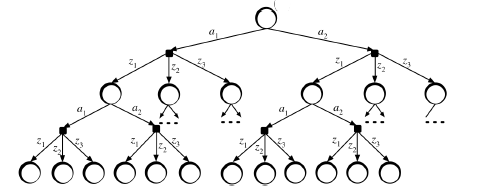
\includegraphics[width=0.6\textwidth]{2.png}
\end{figure}
To compute value at the root:
\begin{itemize}
	\item Initialize leaf with value estimates (or zeroes)
	\item At observation nodes, compute the expected values of the children
	\item At action nodes, compute the max of the children
\end{itemize}
The tree size is $|A|^D|S|^D$. If we use sparse sampling, i.e. we estimate a observation node by only sampling $k$ observations, instead of using all $|S|$ possible observation states, the tree size will be reduced to $|A|^Dk^D$. This solves the exponential growth wrt to the number states, but its growth rate is still exponential to the search depth.
\end{definition}
\begin{definition}[Monte Carlo Tree Search]
\hfill\\\normalfont Monte Carlo Tree Search consists of 4 stages, namely selection, expansion, simulation and backpropagation.
\begin{figure}[h]
\centering
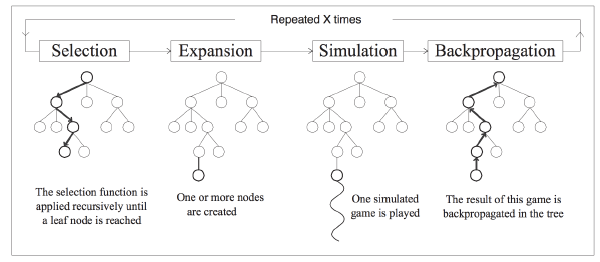
\includegraphics[width=0.6\textwidth]{3.png}
\end{figure}
MCTS repeatedly run trials from the root, where a trial
\begin{itemize}
	\item Repeatedly selet node to go to at next level, until
	\begin{itemize}
		\item target depth reached, or
		\item selected node has not been discovered: then create a new one node, and run a simulation using a default policy till required depth
	\end{itemize}
	\item Back up the outcomes all the way to the root
\end{itemize}
This is an anytime policy: when time is up, it uses the action that looks best at the root at that time.
\end{definition}
For MDP, a tree (actually DAG) node $n$ is associated with a state $s$. A node $n'$ at the next level is selected by applying an action $a$ to $s$, then sampling the next state $s'$ according to $p(s'\mid s,a)$. Here, this action $a$ should be selected by balancing exploration with exploitation.\\
The estimated value $\hat{V}(n)$ at a node $n$ is the avergage reutn of all the trials at $n$. The return $r_t(n)$ of trial $t$ starting from $n$ with state $s$ and next node $n'$ is $R(s)+\gamma r_t(n')$.\\
The estimated $Q$-function(action value function) at $n$, $\hat{Q}(n,a)$ is the average return of all trials at $n$ that starts with action $a$. Therefore, $\hat{Q}(r,a)$ is used to select the action to take at the root.\\
All these functions are updated in the back up operation to the root.
\begin{theorem}[Upper Confidence Tree]
\hfill\\\normalfont UCT uses the following function to select action to go to at node $n$:
\[
\pi_{UCT}(n)=\arg\max_a(\hat{Q}(n,a)+c\sqrt{\frac{\ln(N(n))}{N(n,a)}}
\]
where $N(n)$ is the number of trials through $n$ and $N(n,a)$ is the number of trials through $n$ and $a$. $c$ is a constant, tuned to do well on the problem.\\
It is guaranteed that UCT will converge to optimal policy with enough trials($\Omega(\underbrace{\exp(\exp(\cdots exp(}_{D-1}1)))))$). 
\end{theorem}
\subsection{POMDP}
For Partially Observable Markov Decision Process(POMDP), we no longer observe the state but receive some sensor information that can be used for state estimation.\\
A POMDP has the same elements as an MDP, state $S$, actions $A$, transitions $T$ and reward $R$.\\
In addition, it has observation or sensor model defined by $P(e\mid s)$, the probability of perceiving evidence $e$ given $s$.\\
Since we do not know actual state of the system, we need to track the \textbf{probability distribution} over possible states. We call this \textbf{belief state}, or belief. Belief is updated via the following equation:
\[
b'(s')=\alpha P(e\mid s')\sum_{s}P(s'\mid s,a)b(s)
\]
where $b(s)$ is the current belief, agent does action $a$, and receives evidence $e$, and $\alpha$ is the normalising constant so that $b'$ sums to $1$. This function is written as $b'=\textsc{Forward}(b,a,e)$.\\\
Note, the belief contains all the information necessary for the agent to act optimally; the optimal action depends only on the agent's current belief. Optimal policy can be described as a mapping $\pi^\ast(b)$ from belief to action.\\
The POMDP agent acts as follows:
\begin{itemize}
	\item Given current belief $b$, execute action $a=\pi^\ast(b)$.
	\item Receive the observation $e$
	\item Set the belief to $\textsc{Forward}(b,a,e)$ and repeat.
\end{itemize}
A POMDP can be viewed as a \textit{belief space} MDP:
\begin{itemize}
	\item Define reward function in belief space can be defined as
	\[
\rho(b)=\sum_s b(s)R(s)
	\]
	\item Can derive $P(b'\mid b,a)$ from underlying POMDP.
	\item Taken together $P(b'\mid b,a)$ and $\rho(b)$ defines an observable MDP in belief space.
	\item Optimal policy for this MDP, $\pi^\ast(b)$ is also an optimal policy for the POMDP.
\end{itemize}
However, the belief space is continuous, so we have a continuous MDP, and this results that value and policy iteration algorithms described in MDP cannot be used any more.
\begin{theorem}[Value Iterations for POMDPs]
\hfill\\\normalfont A policy at belief $b_0$ is a conditional plan. Multiple conditional plans are possible. We will have an utility $\alpha_p(s)$ by executing a fixed conditional plan $p$ from a state $s$. Therefore, executing from belief $b$ will have expected utility $\sum_s b(s)\alpha_p(s)$.\\
The potimal policy at a particular belief $b$, is to chooser the conditional plan with highest utility
\[
U(b)=\max_p b\cdot \alpha_p
\]
For finite depth, there is only a finite number of conditional plans. With $|A|$ actions and $|E|$ observations, there are $|A|^{O(|E|)^{d-1}}$ distinct depth-d plans.
\end{theorem}
The continuous belief space is divided into regions, each corresponding to a conditional plan optimal for that region. Here, $U(b)$ is piecewise linear and convex.\\
The value iteration formula is
\[
\alpha_p(s)=R(s)+\gamma(\sum_{s'}P(s'\mid s,a)\sum_{e}P(e\mid s')\alpha_{p,e}(s'))
\]
This gives rise tothe value iteration algorithm:
\begin{theorem}[Value Iteration Algorithm]
\hfill\\\normalfont
\textbf{function} \textsc{POMDP-Value-Iteration}(\textit{pomdp}, $\varepsilon$) \textbf{returns} a utility function\\
\ind \textbf{inputs}: \textit{pomdp}, a POMDP with state $S$, actions $A(s)$ and transition model $P(s'\mid s,a)$.\\
\ind\ind\ind sensor model $P(e\mid s)$, reward $R(s)$ and discount $\gamma$.\\
\ind \ind\ind $\varepsilon$, the maximum error allowed in the utility of any state\\
\ind \textbf{local variables}: $U, U'$ sets of plans $p$ with associated utility vectors $\alpha_p$\\

\ind \textbf{repeat}\\
\ind \ind $U\leftarrow U'$\\
\ind \ind $U'\leftarrow$ the set of all plans consisting of an action and, for each possible next percept, a plan in $U$ with utility vector computed according to equation above\\
\ind \ind $U'\leftarrow$\textsc{Remove-Dominated-Plans}$(U')$\\
\ind \textbf{until} \textsc{Max-Difference}$(U,U')<\varepsilon(1-\gamma)/\gamma$\\
\ind \textbf{return} $U$\\
\end{theorem}
Do note that exact POMDP solvers only work for very space problems. Therefore, online search tend to scale better.\\
Essentially, the execution of POMDP over time can be represented as a \textbf{dynamic decision network}(DDN). POMDP solvers need to solve two problems:
\begin{itemize}
\item Belief tracking
\item Planning problem
\end{itemize}
\begin{definition}[POMCP]
\hfill\\\normalfont Essentially, POMCP is to run UCT on POMDP. To do this, we need to represent beliefs in the nodes.\\
In POMCP, instead of propagating belief forward in a trial, POMCP samples a state at the root from initiall belief, then runs simulation using the state to generate action-observation history. Therefore, it only needs to sample from $p(s'\mid s,a)$ then $p(e\mid s')$ to generate observation $e$ for the action-observation history.
\end{definition}
Another algorithm is DESPOT.
\clearpage
\section{Reinforcement Learning}
Consider the game where an agent can learn the transition model for its own move and possibly to predict opponent move; but the agent often do not get feedback on whether it has done weel until the end of the game.\\
The feedback on whether something good or bad happens is called a \textbf{reward} or \textbf{reinforcement}.\\
We regard reward as part of the input perception, and the agent must be able to recognize it as reward rather than another input.\\
In this section, we assume environment is Markov Decision Process. An optimal policy is a policy that maximizes expected total reward.\\
\textbf{Reinforcement learning} aims to use observed rewards to learn an optimal policy for the environment. Here, we assume agent has no knowledge of the model for environement or reward function.
\subsection{Passive Reinforcement Learning}
In passive learning, policy $\pi$ is fixed, so agent always execute $\pi(s)$ in state $s$. The goal is to learn
\begin{itemize}
	\item Value function $U^{\pi}(s)$ from observations, where
	\item \textbf{transition model} $P(s'\mid s,a)$ and \textbf{reward function} $R(s)$ are unknown.
\end{itemize}
In fact, if transition and reward functions are known, we can just perform policy evaluation.\\
In passive reinforcement learning, the agent executes a set of \textbf{trials} using $\pi$, which can be traced as a sequence of (state, reward) pairs.\\
The utility, or value of $\pi$ at a state $s$ is $U^{\pi}(s)=E[\sum_{t=0}^\infty \gamma^tR(S_t)]$.
\begin{definition}[Adaptive Dynamic Programming]
\hfill\\\normalfont\textbf{Adaptive Dynamic Programming} learns the model, then solves it:
\begin{itemize}
\item Learn transition probabilities $P(s'\mid s, a)$;
\item Learn reward function $R(s)$
\item Calculate value $U^{\pi}(s)$ by solving the Bellman equations.
\end{itemize}
Agent can use \textbf{modified policy iteration} method of doing $k$ iterations of value updates after each change to model.\\
The algorithm is outlined as below:
\textbf{function} \textsc{Passive-ADP-Agent}(\textit{percept}) \textbf{returns} an action\\
\ind \textbf{inputs}: \textit{percept}, a percept indicating the current state $s'$ and reward signal $r'$\\
\ind \textbf{persistent}: $\pi$, a fixed policy\\
\ind \ind \ind \ind \textit{mdp}, an MDP with model $P$, reward $R$, discount $\gamma$\\
\ind \ind \ind \ind $U$, a table of utilities , initially empty\\
\ind \ind \ind \ind $N_{sa}$, a table of frequencies of state-action pairs, initially zero\\
\ind \ind \ind \ind $N_{s'\mid sa}$, a table of outcome frequencies given state action pairs, initially zero\\
\ind \ind \ind \ind $s,a$, the previous state and action, initially null\\
\ind \textbf{if} $s'$ is new \textbf{then} $U[s']\leftarrow r'$, $R[s']\leftarrow r'$\\
\ind \textbf{if} $s$ is not null \textbf{then}\\
\ind \ind increment $N_{sa}[s,a]$ and $N_{s'\mid s,a}[s', s, a]$\\
\ind \ind \textbf{for each} $t$ such that $N_{s'\mid sa}[t,s,a]$ is nonzero \textbf{do}\\
\ind \ind \ind $P(t\mid s,a)\leftarrow N_{s'\mid s,a}[t,s,a]/N_{sa}[s,a]$\\
\ind $U\leftarrow \textsc{Policy-Evaluation}(\pi, U, \textit{mdp})$\\
\ind \textbf{if} $s'.\textsc{Terminal?}$ \textbf{then} $s,a\leftarrow$ null \textbf{else} $s,a\leftarrow s', \pi[s']$.\\
\ind \textbf{return} $a$
\end{definition}
In a state, the utility or value is the \textbf{expected total reawrd} from that state onwards, also called expected reward-to-go or \textbf{return}.\\
In direct utility estimation, often called \textbf{Monte Carlo learning}, we treat each trial as providing a sample of this quantit for each state visited.\\
So we just keep a running average for each state in a table, and in infinitely many trials, sample average will converge to expected value. Esssentially, utility derived from $k$ returns $G_1(s), \ldots, G_k(s)$ is
\[
U_k(s)=\frac{1}{k}\sum_{i=1}^k G_i(s)
\]
We can rearrange the above equation to be
\[
U_k(s)=U_{k-1}(s)+\frac{1}{k}(G_k(s)-U_{k-1}(s))
\]
where $U_{k-1}(s)$ is the estimate after receiving $k-1$ returns, and we call $G_k(s)-U_{k-1}(s)$ the prediction error for the $k$th return.\\
It is clear that Monte Carlo learning is an instance of \textbf{supervised learning}, where each example has state as input and observed return as output.\\
Its advantages are: simple, and each labelled target(return) is an unbiased estimate.\\
The disadvantages include
\begin{itemize}
	\item Need to wait till the end of episode before learning can be done
	\item Variance can be high as a return is a sum of many rewards over the sequence. The varaince can be controlled if we use the discount factor when calculating reward of trials.
\end{itemize}
\subsection{Temporal Difference Learning}
Temporal difference learning exploits more of the Bellman equation constraints. \\
For a transition from state $s$ to $s'$. TD learning does
\[
U^{\pi}(s)\leftarrow U^{\pi}(s)+\alpha(R(s)+\gamma U^{\pi}(s')-U^{\pi}(s))
\]
where $\alpha$ is the \textbf{learning rate}.\\
Here, 
\begin{itemize}
	\item $U^{\pi}(s)$ increases if $R(s)+\gamma U^{\pi}(s')$ is larger than $U^{\pi}(s)$ and decreases it otherwise.
	\item Therefore, we call $R(s)+\gamma U^{\pi}(s')$ the TD target and $(R(s)+\gamma U^{\pi}(s')-U^{\pi}(s))$ the TD error.
	\item It converges to expected value if $\alpha$ decreases with number of times the state has been visited. For example, $\alpha(n)=O(1/n)$.
\end{itemize}
The exact algorithm is below:\\
\textbf{function} \textsc{Passive-TD-Agent}(\textit{percept}) \textbf{returns} an action\\
\ind \textbf{inputs}: \textit{percept}, a percept indicating the current state $s'$ and reward signal $r'$.\\
\ind \textbf{persistent}: $\pi$, a fixed policy\\
\ind \ind \ind \ind $U$, a table of utilities, initially empty\\
\ind \ind \ind \ind  $N_s$ a table of frequencies of states, initially zerop\\
\ind \ind \ind \ind  $s,a,r$, the previous state, action, reward, initially null\\

\ind \textbf{if} $s'$ is new \textbf{then} $U[s']\leftarrow r'$\\
\ind \textbf{if} $s$ not null \textbf{then}\\
\ind \ind increment $N_s[s]$\\
\ind \ind $U[s]\leftarrow U[s]+\alpha(N_s[s])(r+\gamma U[s']-U[s])$\\
\ind \textbf{if} $s'.\textsc{Terminal?}$ \textbf{then} $s,a,r\leftarrow$null \textbf{else} $s,a,r\leftarrow s',\pi[s'], r'$\\
\ind \textbf{return} $a$

The good thing about Temporal Difference is that 
\begin{itemize}
	\item TD can learn online after each step. MC needs complete episode before learning.
	\item TD target $R(s)+\gamma U^{\pi}(s')$ depends only on one measured reward. However, MC target $G(s)$ depends on sum of many rewards. As a result,
	\begin{itemize}
		\item TD target lower variance, but biased
		\item MC target unbiased, but higher variance
	\end{itemize}
	\item TD usually converges faster than MC in practice
\end{itemize}
Above is 1-step TD, where we perform one-step look ahead.
\begin{definition}[{$n$}-step TD]
\hfill\\\normalfont Let $G_{t:t+n}:=R_t+\gamma R_{t+1}+\cdots+\gamma^{n-1}R_{t+n-1}+\gamma^n \hat{v}(S_{t+n})$ be the $n$-step return where $\hat{v}(S_{t+n})$ is the estimated value at state $S_{t+n}$.\\
In $n$-step TD, it sets $G_{t:t+n}$ as the target for update. \\
When $n$ approaches $\infty$, we get Monte Carlo learning. Therefore, intermediate values of $n$ for $n$-step TD tend to work better.
\end{definition}
\begin{definition}[TD{$(\lambda)$}]
\hfill\\\normalfont Instead of using $n$-step return , one can average over different values of $n$. \\
TD$(\lambda)$ sets the following as the target for update
\[
G_t^{\lambda}=(1-\lambda)\sum_{n=1}^\infty \lambda^{n-1}G_{t:t+n}
\]
It can be computed efficiently using method called \textit{eligibility traces}.\\
It converges to $TD$ as $\lambda\to 0$ and converges to MC as $\lambda\to 1$.
\end{definition}
The difference between adaptive dynamic programming against TD is
\begin{itemize}
	\item ADP learns model then solves for value,
	\item whereas TD, MC does not need a model.
	\item ADP tend to be more data efficient, however
	\item TD does not need to compute expectation and does not need to solve system of linear equations, which in turn is computationally more efficient
\end{itemize}
\subsection{Active Reinforcement Learning}
Greedy ADP is a greedy agent, but it may not converge at the optimal policy. Therefore, we want to make actions in reinforcement learning not only gain reward but also help to learn a better model. As a result, we need to trade off between
\begin{itemize}
	\item Exploitation: maximize value as reflected by current estimate
	\item Exploration: learn more about the model to potentially improve long term well being
\end{itemize}
One simple method is called $\epsilon$-\textbf{greedy exploration}, where it choose a greedy action with probability $1-\epsilon$ and a random action with probability $\epsilon$.\\
A scheme for balancing exploration and exploitation must
\begin{itemize}
\item Try each action in each state an unbounded number of times, so as to avoid a finite probability of missing an optimal action
\item Eventually become greedy so that it is optimal with respect to the true model
\end{itemize}
Such schemes are greedy in the limit of infinite exploration(GLIE). One simple GLIE scheme is to $\epsilon$-greedy exploration with choice of $\epsilon=\frac{1}{t}$.\\
However, the shortcoming is, while GLIE based $\epsilon$-greedy eventually converges, it can be slow. An alternative way is to use greedy action selection with respect to an \textbf{optimistic} estimate of the utility $U^{+}(s)$. \\
One example of $U^{+}$ is to use an exploration function $f(u,n)$ with the following update:
\[
U^{+}(s)\leftarrow R(s)+\gamma \max_a f(\sum_{s'}P(s'\mid s,a)U^{+}(s'), N(s,a))
\]
where $N(s,a)$ is the number of times action $a$ has been tried in state $s$ and exploration function $f(u,n)$ \textit{increasing} with $u$ and decreasing with $n$. 
An example of $f(u,n)$ can be
\[
f(u,n)=\begin{cases} R^{+} & \text{ if }n<N_e,\text{ a threshold}\\ u &\text{ otherwise}\end{cases}
\]
where $R^{+}$ is an optimistic estimate of best possible reward.
\subsubsection{Model Free Learning}
Instead of laerning the utility function, we can learn an action-utility function $Q(s,a)$, the value of doing action $a$ in state $s$. $Q$-values are related to utility values by
\[
U(s)=\max_a Q(s,a)
\]
and the optimal action can be derived from $\arg\max$. Since an agent that learns a $Q$-function does not need a model of the form $P(s'\mid s,a)$ for action selection, and thus is called a \textbf{model-free} method.\\
The $Q$-function similarly satisfies a version of the Bellman equations
\[
Q(s,a)=R(s)+\gamma\sum_{s'}P(s'\mid s,a)\max_{a'}Q(s',a')
\]
If we use ADP to learn, we can learn $P(s'\mid s,a)$ and then use an iterative method to compute the $Q$-function, given the estimated model. \\
\textbf{Remark}: ADP with $Q$-function still need model for learning, but not to take action. We can discard $P$ if we use MC or TD.\\
\begin{theorem}[GLIE {$\epsilon$-greedy} MC Control]
\hfill\\\normalfont We sample episode $k$ using current $Q$-function with $\epsilon$-greedy exploration with $\epsilon=\frac{1}{k}$L $S_1,A_1,R_2,\ldots, S_T$.\\
For each $S_t, A_t$ in the episode,

\begin{align*}
N(S_t,A_t)&\leftarrow N(S_t,A_t)+1\\
Q(S_t,A_t)&\leftarrow Q(S_t,A_t)+\frac{1}{N(S_t,A_t)(G_t-Q(S_t,A_t))}
\end{align*}

\end{theorem}
\begin{theorem}[{$Q$}-learning]
\hfill\\\normalfont Using the TD method instead, we can arrive at $Q$-learning:
\[
Q(s,a)\leftarrow Q(s,a)+\alpha(R(s)+\gamma \max_{a'}Q(s', a')-Q(s,a))
\]
\textbf{function} \textsc{Q-Learning-Agent}(\textit{percept}) \textbf{returns} an action\\
\ind \textbf{inputs}: \textit{percept}, a percept indicating the current state $s'$ and reward signal $r'$\\
\ind \textbf{persistent}: $Q$, a table of action values indexed by state and action, initially zero\\
\ind \ind \ind \ind $N_{sa}$, a table of frequencies for state-action pairs, initially zero\\
\ind \ind \ind \ind $s,a,r$, the previous state, action and reward, initially null\\

\ind \textbf{if} \textsc{Terminal?}($s$) \textbf{then} $Q[s,None]\leftarrow r'$\\
\ind \textbf{if} $s$ is not null \textbf{then}\\
\ind \ind increment $N_{sa}[s,a]$\\
\ind \ind $Q[s,a]\leftarrow Q[s,a]+\alpha(N_{sa}[s,a])(r+\gamma \max_{a'}Q[s',a']-Q[s,a])$\\
\ind $s,a,r\leftarrow s', \arg\max_{a'} f(Q[s', a'], N_{sa}[s', a']),r'$\\
\ind \textbf{return} $a$
\end{theorem}
\begin{theorem}[SARSA(State-Action-Reward-State-Action)]
\hfill\\\normalfont SARSA is a slight modification from Q-learning with the update rule being
\[
Q(s,a)\leftarrow Q(s,a)+\alpha(R(s)+\gamma Q(s',a')-Q(s,a))
\]
where $a'$ is the action actually taken.
\end{theorem}
The advantage of SARSA is \textbf{on-policy}. If agent policy is always exploring, it will learn to take that into account. In contrast, $Q$-learning is \textbf{off-policy}, which works regardless of policy for generating trajectories. Therefore, random policy can be used as input too.\\
When greedy agent in SARSA takes action with best $Q$ value, the two will be identical.
\subsection{Function Approximation}
The learning above all require some form of tabular. However, this is not possible if we have many state variables, with respect to which the number of states grows exponentially. \\
One common solution is to use \textbf{function approximation} to represent utility and $Q$-function. For example, we can represent evaluation function as a linear function of \textbf{features}:
\[
\hat{U}_{\theta}(s)=\sum_{i=1}^n \theta_if_i(s)
\]
Here, the $n$ parameters in $\theta$ is used in the function approximation, and the reinforcement learning agent now learns only $\theta$.\\
For Monte Carlo learning, we need to obain a set of training samples $((x_i,y_i), u_i)$ where $u_i$ is the measured utility of the $j$th example. This gives a \textbf{supervised learning problem} since it reduces to a linear regression problem.\\
To minimize the squared error, using online learning, we can, for the $j$th example, take a step in directino of gradient of
\[
E_j(s):=\frac{1}{2}(\hat{U}_\theta(s)-u_j(s))^2
\]
For parameter $\theta_i$, we update via
\[
\theta_i\leftarrow \theta_i-\alpha \frac{\partial E_j(s)}{\partial \theta_i}=\theta_i+\alpha(u_j(s)-\hat{U}_\theta(s))\frac{\partial \hat{U}_\theta(s)}{\partial \theta_i}
\]
The same online learning can be applied to temporal difference learning and $Q$-learning, with the equation adjusted:
\begin{itemize}
	\item For TD:
	\[
\theta_i\leftarrow \theta_i+\alpha[R(s)+\gamma\hat{U}_\theta(s')-\hat{U}_\theta(s)]\frac{\partial \hat{U}_\theta(s)}{\partial \theta_i}
	\]
	\item For $Q$-learning,
	\[
\theta_i\leftarrow \theta_i+\alpha[R(s)+\gamma\max_{\alpha'}\hat{Q}_\theta(s',a')-\hat{Q}_\theta(s,a)]\frac{\partial \hat{Q}_\theta(s,a)}{\partial \theta_i}
	\]
\end{itemize}
This is called \textit{semi}-gradient methods since target is not true value but also depends on $\theta$.\\
For passive TD learning, update rule converges to best approximation of \textbf{linear function}, whereas for active and non-linear functions, there is no guarantee of convergence.
\subsection{Policy Search}
A policy $\pi$ is a mapping from state to action. Assume that the policy is parameterized by some parameters $\theta$. To be useful, the dimension of $\theta$ should be much smaller than number of states.\\
To derive the policy, we can use the $Q$-function:
\[
\pi(s)=\arg\max_a\hat{Q}_\theta(s,a)
\]
\textbf{Policy search} then just adjusts $\theta$ to improve the policy.\\
\textbf{Remark}: If $Q^\ast$ is optimal $Q$-function, $\frac{Q^\ast}{10}$ also works optimally. Therefore, policy search is more flexible than $Q$-learning with functional approximation, as the latter tries to find a value of $\theta$ that $\hat{Q}_\theta$ is \textbf{close} to $Q^\ast$.\\
The problem is when actions are discrete, the policy will also be continuous as a function of $\theta$, which makes gradient-based search difficult. Therefore, we offen use \textbf{stochastic policy} $\pi_\theta(s,a)$ that specifies the probability of selecting action $a$ in state $s$. For example, the softmax function:
\[
P(s,a\mid \pi_\theta)=\frac{e^{\hat{Q}_\theta(s,a)}}{\sum_{a'}e^{\hat{Q}_\theta(s,a')}}
\]
If we can specify the policy value, denoted by $\rho(\theta)$, we can try optimizing for the value. One way is to take a step in the direction of the policy gradient vector $\nabla_\theta \rho(\theta)$ if $\rho(\theta)$ is differentiable. Then we update until we reach an local optimum.\\
In stochastic environment or policy $\pi_\theta(s,a)$, it is possible to obtain an unbiased estimate of gradient at $\theta$,i.e. $\nabla_\theta \rho(\theta)$ directly from results of trials executed at $\theta$.\\
In the case of single action $a$ from single state $s_0$, the gradient is 
\[
\nabla_\theta \rho(\theta)=\nabla_\theta\sum_{a}\pi_\theta(s_0,a)R(a)=\sum_{a}(\nabla_\theta \pi_\theta(s,a))R(a)
\]
We then approximate the summation using samples generated from $\pi_\theta(s_0,a)$:
\[
\nabla_\theta\rho(\theta)=\sum_a \pi_\theta(s_0,a)\frac{(\nabla_\theta \pi_\theta(s,a))R(a)}{\pi_\theta(s_0,a)}\approx \frac{1}{N}\sum_{j=1}^n \frac{(\nabla_\theta\pi\theta(s_0,a_j))R(a_j)}{\pi_\theta(s_0, a_j)}
\]
For sequential case, this generalizes to
\[
\nabla_\theta\rho(\theta)\propto \sum_s p_{\pi_\theta}(s)\sum_{a}\frac{\pi_\theta(s,a)\nabla_\theta\pi_\theta(s,a) Q_{\pi_\theta}(s,a)}{\pi_\theta(s,a)}\approx \frac{1}{N}\sum_{j=1}^n \frac{(\nabla_\theta\pi_\theta(s,a_j))G_j(s)}{\pi_\theta(s,a_j)}
\]
for each state $s$ visited, where $a_j$ is executed in $s$ on $j$th trials and $G_j(s)$ is the total reward received from state $s$ onwards on $j$th trial. \\
We can arrive at REINFORCE algorithm using an online update:
\[
\theta_{j+1}=\theta_j+\alpha G_j\frac{\nabla_\theta\pi_\theta(s,a_j)}{\pi_\theta(s,a_j)}=\theta_j+\alpha G_j\nabla_\theta\ln\pi_\theta(s,a_j)
\]
Should we want to reduce variance, we can do this transformation $Q_{\pi_\theta}(s,a)\to Q_{\pi_\theta}(s,a)-B(s)$. 
\end{document}